%% Beginning of file 'sample631.tex'
%%
%% Modified 2022 May  
%%
%% This is a sample manuscript marked up using the
%% AASTeX v6.31 LaTeX 2e macros.
%%
%% AASTeX is now based on Alexey Vikhlinin's emulateapj.cls 
%% (Copyright 2000-2015).  See the classfile for details.

%% AASTeX requires revtex4-1.cls and other external packages such as
%% latexsym, graphicx, amssymb, longtable, and epsf.  Note that as of 
%% Oct 2020, APS now uses revtex4.2e for its journals but remember that 
%% AASTeX v6+ still uses v4.1. All of these external packages should 
%% already be present in the modern TeX distributions but not always.
%% For example, revtex4.1 seems to be missing in the linux version of
%% TexLive 2020. One should be able to get all packages from www.ctan.org.
%% In particular, revtex v4.1 can be found at 
%% https://www.ctan.org/pkg/revtex4-1.

%% The first piece of markup in an AASTeX v6.x document is the \documentclass
%% command. LaTeX will ignore any data that comes before this command. The 
%% documentclass can take an optional argument to modify the output style.
%% The command below calls the preprint style which will produce a tightly 
%% typeset, one-column, single-spaced document.  It is the default and thus
%% does not need to be explicitly stated.
%%
%% using aastex version 6.3
\documentclass[preprint]{aastex631}
\usepackage{amsmath}
\usepackage{subfigure}
%% The default is a single spaced, 10 point font, single spaced article.
%% There are 5 other style options available via an optional argument. They
%% can be invoked like this:
%%
%% \documentclass[arguments]{aastex631}
%% 
%% where the layout options are:
%%
%%  twocolumn   : two text columns, 10 point font, single spaced article.
%%                This is the most compact and represent the final published
%%                derived PDF copy of the accepted manuscript from the publisher
%%  manuscript  : one text column, 12 point font, double spaced article.
%%  preprint    : one text column, 12 point font, single spaced article.  
%%  preprint2   : two text columns, 12 point font, single spaced article.
%%  modern      : a stylish, single text column, 12 point font, article with
%% 		  wider left and right margins. This uses the Daniel
%% 		  Foreman-Mackey and David Hogg design.
%%  RNAAS       : Supresses an abstract. Originally for RNAAS manuscripts 
%%                but now that abstracts are required this is obsolete for
%%                AAS Journals. Authors might need it for other reasons. DO NOT
%%                use \begin{abstract} and \end{abstract} with this style.
%%
%% Note that you can submit to the AAS Journals in any of these 6 styles.
%%
%% There are other optional arguments one can invoke to allow other stylistic
%% actions. The available options are:
%%
%%   astrosymb    : Loads Astrosymb font and define \astrocommands. 
%%   tighten      : Makes baselineskip slightly smaller, only works with 
%%                  the twocolumn substyle.
%%   times        : uses times font instead of the default
%%   linenumbers  : turn on lineno package.
%%   trackchanges : required to see the revision mark up and print its output
%%   longauthor   : Do not use the more compressed footnote style (default) for 
%%                  the author/collaboration/affiliations. Instead print all
%%                  affiliation information after each name. Creates a much 
%%                  longer author list but may be desirable for short 
%%                  author papers.
%% twocolappendix : make 2 column appendix.
%%   anonymous    : Do not show the authors, affiliations and acknowledgments 
%%                  for dual anonymous review.
%%
%% these can be used in any combination, e.g.
%%
%% \documentclass[twocolumn,linenumbers,trackchanges]{aastex631}
%%
%% AASTeX v6.* now includes \hyperref support. While we have built in specific
%% defaults into the classfile you can manually override them with the
%% \hypersetup command. For example,
%%
%% \hypersetup{linkcolor=red,citecolor=green,filecolor=cyan,urlcolor=magenta}
%%
%% will change the color of the internal links to red, the links to the
%% bibliography to green, the file links to cyan, and the external links to
%% magenta. Additional information on \hyperref options can be found here:
%% https://www.tug.org/applications/hyperref/manual.html#x1-40003
%%
%% Note that in v6.3 "bookmarks" has been changed to "true" in hyperref
%% to improve the accessibility of the compiled pdf file.
%%
%% If you want to create your own macros, you can do so
%% using \newcommand. Your macros should appear before
%% the \begin{document} command.
%%
\newcommand{\vdag}{(v)^\dagger}
\newcommand\aastex{AAS\TeX}
\newcommand\latex{La\TeX}

%% Reintroduced the \received and \accepted commands from AASTeX v5.2
%\received{March 1, 2021}
%\revised{April 1, 2021}
%\accepted{\today}

%% Command to document which AAS Journal the manuscript was submitted to.
%% Adds "Submitted to " the argument.
%\submitjournal{PSJ}

%% For manuscript that include authors in collaborations, AASTeX v6.31
%% builds on the \collaboration command to allow greater freedom to 
%% keep the traditional author+affiliation information but only show
%% subsets. The \collaboration command now must appear AFTER the group
%% of authors in the collaboration and it takes TWO arguments. The last
%% is still the collaboration identifier. The text given in this
%% argument is what will be shown in the manuscript. The first argument
%% is the number of author above the \collaboration command to show with
%% the collaboration text. If there are authors that are not part of any
%% collaboration the \nocollaboration command is used. This command takes
%% one argument which is also the number of authors above to show. A
%% dashed line is shown to indicate no collaboration. This example manuscript
%% shows how these commands work to display specific set of authors 
%% on the front page.
%%
%% For manuscript without any need to use \collaboration the 
%% \AuthorCollaborationLimit command from v6.2 can still be used to 
%% show a subset of authors.
%
%\AuthorCollaborationLimit=2
%
%% will only show Schwarz & Muench on the front page of the manuscript
%% (assuming the \collaboration and \nocollaboration commands are
%% commented out).
%%
%% Note that all of the author will be shown in the published article.
%% This feature is meant to be used prior to acceptance to make the
%% front end of a long author article more manageable. Please do not use
%% this functionality for manuscripts with less than 20 authors. Conversely,
%% please do use this when the number of authors exceeds 40.
%%
%% Use \allauthors at the manuscript end to show the full author list.
%% This command should only be used with \AuthorCollaborationLimit is used.

%% The following command can be used to set the latex table counters.  It
%% is needed in this document because it uses a mix of latex tabular and
%% AASTeX deluxetables.  In general it should not be needed.
%\setcounter{table}{1}

%%%%%%%%%%%%%%%%%%%%%%%%%%%%%%%%%%%%%%%%%%%%%%%%%%%%%%%%%%%%%%%%%%%%%%%%%%%%%%%%
%%
%% The following section outlines numerous optional output that
%% can be displayed in the front matter or as running meta-data.
%%
%% If you wish, you may supply running head information, although
%% this information may be modified by the editorial offices.
%\shortauthors{Schwarz et al.}
%%
%% You can add a light gray and diagonal water-mark to the first page 
%% with this command:
%% \watermark{text}
%% where "text", e.g. DRAFT, is the text to appear.  If the text is 
%% long you can control the water-mark size with:
%% \setwatermarkfontsize{dimension}
%% where dimension is any recognized LaTeX dimension, e.g. pt, in, etc.
%%
%%%%%%%%%%%%%%%%%%%%%%%%%%%%%%%%%%%%%%%%%%%%%%%%%%%%%%%%%%%%%%%%%%%%%%%%%%%%%%%%
%\graphicspath{{./}{figures/}}
%% This is the end of the preamble.  Indicate the beginning of the
%% manuscript itself with \begin{document}.

\begin{document}

\title{Holographic dark energy models in $f(Q,T)$ gravity and cosmic constraint}

%% LaTeX will automatically break titles if they run longer than
%% one line. However, you may use \\ to force a line break if
%% you desire. In v6.31 you can include a footnote in the title.

%% A significant change from earlier AASTEX versions is in the structure for 
%% calling author and affiliations. The change was necessary to implement 
%% auto-indexing of affiliations which prior was a manual process that could 
%% easily be tedious in large author manuscripts.
%%
%% The \author command is the same as before except it now takes an optional
%% argument which is the 16 digit ORCID. The syntax is:
%% \author[xxxx-xxxx-xxxx-xxxx]{Author Name}
%%
%% This will hyperlink the author name to the author's ORCID page. Note that
%% during compilation, LaTeX will do some limited checking of the format of
%% the ID to make sure it is valid. If the "orcid-ID.png" image file is 
%% present or in the LaTeX pathway, the OrcID icon will appear next to
%% the authors name.
%%
%% Use \affiliation for affiliation information. The old \affil is now aliased
%% to \affiliation. AASTeX v6.31 will automatically index these in the header.
%% When a duplicate is found its index will be the same as its previous entry.
%%
%% Note that \altaffilmark and \altaffiltext have been removed and thus 
%% can not be used to document secondary affiliations. If they are used latex
%% will issue a specific error message and quit. Please use multiple 
%% \affiliation calls for to document more than one affiliation.
%%
%% The new \altaffiliation can be used to indicate some secondary information
%% such as fellowships. This command produces a non-numeric footnote that is
%% set away from the numeric \affiliation footnotes.  NOTE that if an
%% \altaffiliation command is used it must come BEFORE the \affiliation call,
%% right after the \author command, in order to place the footnotes in
%% the proper location.
%%
%% Use \email to set provide email addresses. Each \email will appear on its
%% own line so you can put multiple email address in one \email call. A new
%% \correspondingauthor command is available in V6.31 to identify the
%% corresponding author of the manuscript. It is the author's responsibility
%% to make sure this name is also in the author list.
%%
%% While authors can be grouped inside the same \author and \affiliation
%% commands it is better to have a single author for each. This allows for
%% one to exploit all the new benefits and should make book-keeping easier.
%%
%% If done correctly the peer review system will be able to
%% automatically put the author and affiliation information from the manuscript
%% and save the corresponding author the trouble of entering it by hand.

%\correspondingauthor{August Muench}
%\email{greg.schwarz@aas.org, gus.muench@aas.org}

\author[0000-0002-0786-7307]{Xuwei Zhang}
\affiliation{Xinjiang Astronomical Observatory, Chinese Academy of Sciences, 150 Science 1-Street,Urumqi 830011, China}
\affiliation{University of Chinese Academy of Sciences, Beijing 100049, China}

\author[0000-0002-0786-7307]{Xiaofeng Yang}
\affiliation{Xinjiang Astronomical Observatory, Chinese Academy of Sciences, Urumqi 830011, China}
\affiliation{University of Chinese Academy of Sciences, Beijing 100049, China}

\author[0000-0002-0786-7307]{Yunliang Ren}
\affiliation{Xinjiang Astronomical Observatory, Chinese Academy of Sciences, Urumqi 830011, China}
\affiliation{School of Physical Science and Technology, Xinjiang University, 666 Shenli Street, 830046 Urumqi, China}

\author[0000-0002-0786-7307]{Shuangnan Chen}
\affiliation{Xinjiang Astronomical Observatory, Chinese Academy of Sciences, Urumqi 830011, China}
\affiliation{School of Physical Science and Technology, Xinjiang University, 666 Shenli Street, 830046 Urumqi, China}

\author[0000-0002-0786-7307]{Yangjun Shi}
\affiliation{Xinjiang Astronomical Observatory, Chinese Academy of Sciences, Urumqi 830011, China}
\affiliation{School of Physics and Astronomy, China West Normal University, Nanchong 637002, China}

\begin{abstract}
In this work, we investigate a modified gravity model \( f(Q,T) \) with holographic dark energy. By considering the holographic principle as an extension to cosmology, we explore dark energy as a result of the entanglement entropy of the universe's horizon. We employ the Barrow holographic dark energy model, incorporating quantum corrections, and use the Hubble horizon for the infrared cutoff. Through parameter estimation using MCMC with the latest supernova, BAO, and Hubble data, we find that the model alleviates the Hubble tension and provides consistent results with the standard cosmological model. Additionally, the model successfully describes the accelerated expansion of the universe. Despite the complexity and additional parameters introduced by the model, it offers a promising framework for further exploration of dark energy within modified gravity theories.
\end{abstract}

%% Keywords should appear after the \end{abstract} command. 
%% The AAS Journals now uses Unified Astronomy Thesaurus concepts:
%% https://astrothesaurus.org
%% You will be asked to selected these concepts during the submission process
%% but this old "keyword" functionality is maintained in case authors want
%% to include these concepts in their preprints.
\keywords{Cosmology, Dark energy}

%% From the front matter, we move on to the body of the paper.
%% Sections are demarcated by \section and \subsection, respectively.
%% Observe the use of the LaTeX \label
%% command after the \subsection to give a symbolic KEY to the
%% subsection for cross-referencing in a \ref command.
%% You can use LaTeX's \ref and \label commands to keep track of
%% cross-references to sections, equations, tables, and figures.
%% That way, if you change the order of any elements, LaTeX will
%% automatically renumber them.
%%
%% We recommend that authors also use the natbib \citep
%% and \citet commands to identify citations.  The citations are
%% tied to the reference list via symbolic KEYs. The KEY corresponds
%% to the KEY in the \bibitem in the reference list below. 

\section{Introduction} \label{sec:intro}
Over the past decaeds, a series of discoveries in cosmology have profoundly changed our understanding of the universe. In 1998, the accelerated expansion of the universe was discovered through the study of Type Ia supernovae(\cite{perlmutter_discovery_1998,Riess_1998}). This fact had been later confirmed by many other cosmological observations, such as the measurement of temperature anisotropy and polarization in the cosmic microwave background (CMB) radiation(\cite{1992ApJ...396L...1S,2020Planck}); Baryon acoustic oscillations (Baryon Acoustic Oscillations, BAO) peak length scale(\cite{Eisenstein_2005,10.1111/j.1365-2966.2011.19592.x}); the study of the large-scale structure (LSS) of the universe(\cite{Dodelson_2002,Percival_2007}) and use Cosmic Chronometers to direct measurement of Hubble parameter(\cite{Daniel_Stern_2010,Moresco_2015}). These observations suggest the existence of a mysterious energy in our universe, also named dark energy (DE)  who has high negative pressure and increasing density. Dark energy behaves as anti-gravity, but its nature remains unknown.

Theoretical predictions and astronomical observations indicate that there may be a mysterious form of energy in the universe. This energy has the characteristics of negative pressure, and its density increases over time. This is considered to be the key factor driving the accelerated expansion of the universe, accounting for about three-quarters of the total energy of the universe (\cite{PhysRevD.37.3406,PhysRevD.63.103510,10.1143/PTP.106.929}). In order to achieve such accelerated expansion, this form of energy needs to produce an anti-gravitational effect throughout the observable universe. However, ordinary baryonic matter neither has this equation of state nor can it explain such a large proportion of the cosmic energy component. Therefore, scientists have proposed and studied a variety of alternative theories and models to explore the nature of this cosmic acceleration phenomenon.

The simplest and most widely accepted theory is $\Lambda \text{CDM}$ model, where $\Lambda$ means cosmological constant predicted by Einstein(\cite{Carroll_2001}).
Based on $\Lambda \text{CDM}$ model, the lastest observations suggest that our universe consists of 68.3\% dark energy, 26.8\% cold dark matter and 4.9\% ordinary matter (\cite{2020Planck}). However, this model is not free from problems and the problems it is facing are cosmic coincidence, fine-tuning and the Hubble tension—a discrepancy between the value of the Hubble constant $H_0$ inferred from the CMB by the Planck satellite and that obtained from local measurements using Type Ia supernovae—has sparked significant debate. 

Another interesting attempt is to deviate from general ralativity toward a modified form (detailed research progress can be reviewid in \cite{Clifton_2012}). These theories assume that general relativity not work in large scale requiring a modification in action rather than standard Einstein-Hilbert action. The most well-known is $F(R)$ gravity which replaces the Ricci scalar $R$ in the action by a general function $f(R)$ (\cite{1970MNRAS.150....1B}). The $f(G)$ gravity theory is also a modified theory of gravity that introduces a correction to the Gauss–Bonnet (GB) term $G$, allowing it to be arbitrary function $f(G)$ rather than remaining a constant(\cite{NOJIRI20051,NOJIRI_2007}). Another modified theory of gravity $f(T)$ extends the teleparallel equivalent of General Relativity (TEGR). It replaces the curvature scalar $R$ in action with the torsion scalar $T$, derived from the Weitzenböck connection. Also shows some interpretations for the accelerating phases of our Universe(\cite{Cai_2016,Bengochea_2009}). $f(Q)$ is generalized symmetric teleparallel gravity, with curvature and torsion both being zero, which is inspired by Weyl and Einstein's trial to unify electromagenetic and gravity. The geometric properties of gravity are described by "non-metricity". That is, the covariant derivative of the metric tensor is no longer zero (some detailed information can be found in review \cite{HEISENBERG20241}). Harko et al. have proposed a new theory known as $f (R, T )$ gravity, where $R$ stands for the Ricci scalar and $T$ denotes the trace of energy-momentum tensor which presents a non-minimum coupling between geometry and matter(\cite{PhysRevD.84.024020}). Similar theories are introduced,$f(R,G)$ gravity proposed by Bamba et al.(\cite{Bamba2009FinitetimeFS}); $f(Q,T)$ proposed by Xu et al.(\cite{Xu_2019}); $f(Q,C)$ gravity(\cite{De_2024}); $f(\mathcal{T},T)$ proposed by(\cite{Harko_2014}); $f(T,B)$ gravity(\cite{Bahamonde_2015,Bahamonde_2017}); $f(R,T^2)$ proposed by Katırcı et al.(\cite{Kat_rc__2014}), etc.

Holographic dark energy is an famous alternative theory for the interpretation of dark energy, originating from the holographic principle proposed by ’t Hooft(\cite{hooft2009dimensionalreductionquantumgravity}). Cohen et al. introduced the "UV-IR" relationship, highlighting that in effective quantum field theory, a system of size $L$ has its entropy and energy constrained by the Bekenstein entropy bound and black hole mass, respectively. This implies that quantum field theory is limited to describing low-energy physics outside black holes(\cite{cohen_effective_1999}). After that, Li et al. proposed that the infrared cut-off relevant to the dark energy is the size of the event horizon and obtained the dark energy density can be described as $\rho_\text{de}=3c^2 M_p^2 R_h^2$ where $R_h$ is future horizon of our universe(\cite{LI20041}). Although choose Hubble cut-off is a natural thought, but Hsu found it might lead to wrong state equation and be strongly disfavored by observational data(\cite{Hsu_2004}).

Various attempts to reconstruct or discuss HDE in modified gravity have been completed by several authors. Wu and zhu reconstructed HDE in $f(R) $ gravity (\cite{wu_reconstructing_2008}). Shaikh et al. discussed HDE in $f (G)$ gravity with Bianchi type 1 model (\cite{shaikh_holographic_2020}). Zubair et al. reconstructed Tsallis holographic dark energy models in modified $f(T, B)$ gravity (\cite{zubair_reconciling_2021}). Sharif et al. studied the cosmological evolution of HDE in $f(\mathcal{G},T)$ gravity (\cite{sharif_cosmic_2019}) and Alam et al. investigated Renyi HDE in the same gravity (\cite{alam_renyi_2023}). Myrzakulov et al. reconstructed Barrow HDE in $f(Q,T)$ gravity (\cite{myrzakulov_barrow_2024}). Singh et al. and Devi et al. discussed HDE models respectively in $f(R,T)$ gravity and take cosmic constraint (\cite{singh_statefinder_2016,devi_barrow_2024}).


In this article, we assume that our universe is in a $f(Q,T)$ gravity and HDE exists as one component of fluid, we will breifly introduce $f(Q,T)$ gravity and HDE model in section \ref{sec:mghde}.

\section{$f(Q,T)$ gravity theory}\label{sec:mghde}

Weyl in 1918 introduced an extension of Riemannian geometry, using a non-metricity tensor $Q_{\alpha \mu \nu}=\nabla_\alpha g_{\mu \nu}=-w_\alpha g_{\mu \nu}$, which describes how the length of a vector changes during parallel transport where $w_\alpha$ coincides with those of the electromagnetic potentials (\cite{Weyl:1918ib}). Weyl geometry can also be extended to so-called Weyl-Cartan geometry by considering the torsion of spacetime.

In Weyl-Cartan geometry, a connection
can be decomposed into three independent parts: the Christoffel symbol $\hat{\Gamma}^\alpha_{\ \mu \nu}$, the contortion tensor $K^\alpha_{\ \mu \nu}$ and the disformation tensor $L^\alpha_{\ \mu \nu}$, so that the general affine connection can be expressed as (\cite{J_rv_2018})
\begin{equation}
    \Gamma^\alpha_{\ \mu \nu}=\hat{\Gamma}^\alpha_{\ \mu \nu}+K^{\alpha}{}_{\mu \nu}+L^\alpha{}_{\mu \nu}
\end{equation}
whereas
\begin{align}
\hat{\Gamma}^\alpha{}_{\mu \nu}& =\frac{1}{2}g^{\alpha \beta}(\partial_\mu g_{\beta \nu}+\partial_\nu g_{\beta \mu}-\partial_\beta g_{\mu \nu}) \\
K^{\alpha }{}_{\mu \nu }& = \frac{1}{2}T^{\alpha }{}_{\mu \nu }+T_{(\mu}{}^{\alpha }{}_{\nu )} \\
L^{\alpha}{}_{\mu\nu}& = \frac{1}{2}Q^{\alpha}_{}{\mu\nu}-Q_{(\mu}{}^{\alpha }{}_{\nu)}
\end{align}
are the standard Levi-civita connection of metric $g_{\mu \nu}$, contortion and disformation tensors respectively.
In the above definitions, the torsion tensors and the non-metric tensor are introduced as follow
\begin{align}
Q_{\rho \mu\nu} &\equiv \nabla_{\rho} g_{\mu\nu} = \partial_\rho g_{\mu\nu} - \Gamma^\beta{}_{\rho \mu} g_{\beta\nu} - \Gamma^\beta{}_{\rho\nu} g_{\mu\beta}\\
T^{\alpha}{}_{\mu\nu} &\equiv 2\Gamma^{\alpha}{}_{[\mu\nu]} =\Gamma^{\alpha}{}_{\mu\nu}-\Gamma^{\alpha}{}_{\nu\mu}
\end{align}
The non-metric tensor has two independent traces, namely $Q_{\mu}=Q_{\mu}{}^{\alpha}{}_{\alpha}$ and $\tilde{Q}^{\mu}=Q_{\alpha}{}^{\mu \alpha}$, so we can get quadratic non-metricity scalar as
\begin{equation}
    Q=\dfrac{1}{4}Q_{\alpha\beta\mu}Q^{\alpha\beta\mu}-\dfrac{1}{2}Q_{\alpha\beta\mu}Q^{\beta\mu\alpha}-\dfrac{1}{4}Q_{\alpha}Q^{\alpha}+\dfrac{1}{2}Q_{\alpha}\tilde{Q}^\alpha\label{Qscalar} 
\end{equation} 

We consider the general form of the Einstein-Hilbert action for the $f(Q,T)$ gravity in the unit $8\pi G=1$
\begin{equation}
S=\int(\frac{1}{2}f(Q,T)+\mathcal{L}_m) \sqrt{-g}  d^4x \label{action}
\end{equation}
where $f$ is an arbitrary function of the non-metricity , $\mathcal{L}_m$ is known as matter Lagrangian, $g=\det (g_{\mu \nu})$ denotes determinant of metric tensor, and $T=g^{\mu \nu}T_{\mu \nu}$ is the trace of the matter-energy-momentum tensor, where $T_{\mu \nu}$ is defined as
\begin{equation}
    T_{\mu \nu}=-\frac{2}{\sqrt{-g}}\frac{\delta(\sqrt{-g}\mathcal{L}_m)}{\delta g^{\mu \nu}}
\end{equation}
Vary the action \eqref{action} with respect to the metric tensor $g_{\mu\nu}$ we can get
\begin{align}
\delta S&=\int \left(\frac{1}{2} \delta[f(Q,T) \sqrt{-g}]+\delta(\mathcal{L}_m \sqrt{-g})\right)d^4x \\
&= \int \frac{1}{2}\left(-\frac{1}{2}f g_{\mu\nu}\sqrt{-g}\delta g^{\mu\nu}+f_Q \sqrt{-g} \delta Q+f_T \sqrt{-g}\delta T -\frac{1}{2}T_{\mu \nu}\sqrt{-g}\delta g^{\mu\nu}\right)d^4x
\end{align}
In analogy to studies on torsionless $f(R)$ gravity and
curvature-free $f(T)$ gravity, we can generalize the
gravity to theories containing an arbitrary function of
the non-metricity scalar i.e. $f(Q,T)$. Therefore, we con-
sider the following action
\begin{equation}
-\frac{2}{\sqrt{-g}}\nabla_\alpha(f_Q \sqrt{-g}P^\alpha_{\ \ \mu \nu})-\frac{1}{2}f g_{\mu \nu}+f_T(T_{\mu \nu}+\Theta_{\mu \nu})-f_Q(P_{\mu \alpha \beta}Q^\nu_{\ \ \alpha \beta}-2Q^{\alpha \beta}_{\ \ \ \ \mu}P_{\alpha \beta \nu})=T_{\mu \nu}\label{FieldEq}
\end{equation}
Where tensor $\Theta_{\mu \nu}$ are defined as $g^{\alpha\beta}\delta T_{\alpha\beta}/{\delta g^{\mu\nu}}$ and $P^{\alpha}_{\mu\nu}$ is the super-potential of the model (detailed discussion found in \cite{Xu_2019}). In the case of a globally vanishing affine connections, the non-metricity tensor depends on the metric
only and Einstein's GR action is recovered. This occurs
under the choice of the coincidence gauge, in which the
origin of spacetime and that of the tangent space coincide. In the coincident gauge with $\Gamma^{\alpha}_{\mu\nu}=0$ we have $Q=6H^2$ (detailed discussion can be found in \cite{lu2019cosmologysymmetricteleparallelgravity}).

Assuming that the Universe is described by the isotropic, homogeneous and spatially flat Friedmann-Lemaitre-Robertson-Walker (FLRW) spacetime, given by as line element
\begin{equation}
ds^2=-N^2(t)dt^2+a^2(t)\delta_{ij} dx^i dx^j\label{FLRW}
\end{equation}
where $a(t)$ is the cosmic scale factor
used to define the Hubble expansion rate $H=\dot{a}/a$ and the lapse function $N(t)$ used to define dilation rates $\tilde{T}=\dot{N}/N$ (for standard case $N(t)=1$). To derive Friedmann equations describing the cosmological evolution, we assume that the matter content of the Universe consists of a perfect fluid, whose  energy-momentum tensor is given by $T^{\mu}_\nu=\text{diag}(-\rho,p,p,p)$ and tensor $\Theta^{\mu}_\nu$ is expressed as $\text{diag}(2\rho+p,-p,-p,-p)$. Then use the line element \eqref{FLRW} and field equation \eqref{FieldEq}, we can get Friedmann equations
\begin{align}
\rho &=\frac{f}{2}-6f_Q H^2-\frac{2f_T}{1+f_T}(\dot{f}_QH+f_Q \dot{H}) \\
p &=-\frac{f}{2}+6f_Q H^2+2(\dot{f}_QH+f_Q \dot{H})
\end{align}
where $f(Q,T)$ is simplified to $f$, and $f_Q=\partial f/\partial Q$, $f_T=\partial f/\partial T$, $\dot{f}_Q=\partial f_Q/\partial t$. By the usage of Eq. \eqref{Qscalar} and the line element \eqref{FLRW}, there exists following relationship (The detailed derivation can be found in the appendix of \cite{Xu_2019})
\begin{equation}
    Q=6H(t)^2
\end{equation}

The equation of state (EoS) parameter is given by
\begin{equation}
    w=\frac{p}{\rho}=-1+\frac{4 f_Q H+f_Q \dot{H}}{(1+f_T)(f-12f_QH^2)-4 f_T(\dot{f}_QH+f_Q \dot{H})},
\end{equation}
where $\rho$ and $p$ denote the total energy density and pressure of the universe. Since we mainly focus in the late universe, the contribution of radiation can be ignored, so we only care about baryonic matter and holographic dark energy fluid.
\begin{equation}
    \rho=\rho_m+\rho_\text{de}, \quad p=p_m+p_\text{de}
\end{equation}
In our universe, the condition $w < -1/3$ ensures accelerated expansion. 

Effective EoS parameter denote geometry qualities.
\begin{align}
\rho_{\text{eff}}&=3H^2=\frac{f}{4f_Q}-\frac{1}{2f_Q}[(1+f_T)\rho+f_T p] \label{F1}\\
-p_{\text{eff}}&=2\dot{H}+3H^2=\frac{f}{4f_Q}-\frac{2\dot{f}_Q H}{f_Q}+\frac{1}{2f_Q}[(1+f_T)\rho +(2+f_T)p] \label{F2}
\end{align}
The effective energy density \(\rho_{\text{eff}}\) and pressure \(p_{\text{eff}}\) described above highlight the coupling between geometry and matter within the \(f(Q, T)\) gravity framework. The presence of \(f_T\) explicitly links the geometric modifications to the energy density \(\rho\) and pressure \(p\) of the matter content. Additionally, the term involving \(\dot{f}_Q\) introduces time dependence in the coupling, suggesting a dynamical interplay between the evolution of spacetime geometry and matter distribution. 

Furthermore, the effective EoS using Eq.\eqref{F1}\eqref{F2} can be written as
\begin{equation}
w_{\text{eff}}=\frac{p_{\text{eff}}}{\rho_{\text{eff}}} = \frac{-2\dot{H}-3H^2}{3H^2}= -\frac{f - 8\dot{f}_Q H + 2[(1 + f_T)\rho + (2 + f_T)p]}{f - 2[(1 + f_T)\rho + f_T p]}
\end{equation}



\section{Cosmic solutions with holographic dark energy}

The holographic principle sets an upper limit on the entropy of the universe.  In the HDE model, the energy density of dark energy is typically expressed as (\cite{LI20041})
\begin{equation}
    \rho_\text{de} = 3c^2 M_p^2 L^{-2}
\end{equation}
where $L$ is the characteristic length scale of the universe, and $c$ is free parameter, $M_p$ denotes planck mass here we set it as 1. The Hubble horizon is considered the simplest option.  In addition, the particle horizon $L_p$ or the future event horizon $L_F$ are also considered reasonable options. Consider a simple case, the HDE energy density in Hubble cut-off can be described as 
\begin{equation}
    \rho_{de}=3c^2 H(t)^2 \label{HDE}
\end{equation}
Another HDE model called barrow holographic dark energy (BHDE) generalizes holographic entropy that arises from quantum-gravitational effects which deform the black-hole surface by giving it an intricate, fractal form . In this case, the HDE energy density can be define as
\begin{equation}
    \rho_{de}=3c^2 H(t)^{2-\Delta}\label{BHDEdef}
\end{equation}
here a new exponent $\Delta$ quantifies the quantum-gravitational deformation, with $\Delta=0$ coming back to the standard Bekenstein-Hawking entropy, and with $\Delta=1$ corresponding to the most intricate and fractal structure (\cite{PhysRevD.102.123525}).

In order to incorporate holographic dark energy in the modified gravitational universe, we consider a simple form of $f$ 
\begin{equation}
    f(Q,T)=m Q^n+\alpha T
\end{equation}
where $Q=6H^2$, $T=-\rho+3p$, $m$, $n$ and $\alpha$ are constants. So that we can derive $f_Q=\alpha n Q^{n-1}=\alpha n 6^{n-1}H^{2n-2}$, $f_T=\beta$, $\dot{f}_Q=2\alpha n(n-1)6^{n-1}H^{2n-3}\dot{H}$.

We also introduce the deceleration factor, which describes the acceleration or deceleration of the late universe depending upon its value, is defined as
\begin{equation}
    q=\frac{d}{dt}\frac{1}{H}-1=-\frac{\ddot{a}a}{\dot{a}^2}=-\frac{\dot{H}}{H^2}-1=(1+z)\frac{1}{H(z)}\frac{dH(z)}{dz}-1   
\end{equation}
In order to understand the characteristic properties of the dark energy and more easier to get a analytical solution, we need to parameterize EoS of HDE as a constant parameter
\begin{equation}
    w_\text{de}=\frac{p_\text{de}}{\rho_\text{de}}
\end{equation}
Use Eq.\eqref{F1} and \eqref{F2} we can solve the energy density of fluid component in field equation
\begin{align}
    \rho_\text{de}&= \frac{m (2 n-1) \left(6H(t)^2\right)^{n-1} \left((3 \alpha +2) n H'(t)+3 (\alpha +1) H(t)^2\right)}{\left(2 \alpha ^2+3 \alpha +1\right) w_\text{de}} \label{RD}\\
    \rho_m&= \frac{m (2 n-1) \left(6H(t)^2\right)^{n-1} \left(n (\alpha  (w_\text{de}-3)-2) H'(t)-3 (\alpha +1) (w_\text{de}+1) H(t)^2\right)}{\left(2 \alpha ^2+3 \alpha +1\right) w_\text{de}}\label{RM}
\end{align}
This is a second order differential equation and it depends on t. In order to get cosmological solution, there is also a simple relation between $H(t)$ and $H(z)$
\begin{equation}
    \dot{H}(t)=\frac{d}{dt}H(t)=-\frac{d H(z)}{dz}H(z)(1+z)\label{HR}
\end{equation}
Combine equation \eqref{RD} \eqref{RM} and \eqref{HR} and relation \eqref{HR}, we can get the equation follows
\begin{equation}
    3 c^2 H(z)^2=\frac{m 6^{n-1} (2 n-1) \left(H(z)^2\right)^{n-1} \left(3 (\alpha +1) H(z)^2-(3 \alpha +2) n (z+1) H(z) H'(z)\right)}{\left(2 \alpha ^2+3 \alpha +1\right) {w_\text{de}}}
\end{equation}
% We first not consider non-minimum coupling between geometry and matter assuming that $\alpha=0$, so that we don't need to talk the dynamic tensor coupling terms $T$. To get an analytic form, we also assume that $n=1$, so we can get
% \begin{equation}
%     H(z) = H_0  (1+z)^{\frac{3}{2}-\frac{3 c^2 w_\text{de}}{2 m}}
% \end{equation}

% \begin{equation}
%     H(z)= H_0(z+1)^{3/2}-c^2 w_\text{de}((1+z)^{3/2}-1)\frac{1}{m}
% \end{equation}
In principle, we can get the form of $H(z)$ through the solution of above differential equation. However, solving higher-order differential equations analytically is difficult. So we consider $n=1$ firstly to simplify calculation and set the initial condition $H(z=0)=H_0$ which denotes value of the Hubble parameter at present, get analytically solution as follow
\begin{equation}
    H(z)= H_0 (1+z)^{\frac{3 (1+\alpha) \left(m-c^2 w_\text{de}(1+2\alpha)\right)}{m(2+3\alpha)}}
\end{equation}
We thus obtain the power-law evolution of the Universe which avoids the big-bang singularity similar to the $f(R,T)$ situation in (\cite{singhStatefinderDiagnosisHolographic2016}). In this case, the deceleration factor is
\begin{equation}
    q = -1+\frac{3 (\alpha +1) \left(m-(2 \alpha +1) c^2 w_\text{de}\right)}{(3 \alpha +2) m}
\end{equation}
Here we have a constant deceleration factor depending on the parameter. When we select a particular parameter value, it will show acceleration or deceleration characteristics. If $q<0$, it will show the characteristics of accelerated expansion. However, since the deceleration factor is time independent, there is no phase transition in such a universe. So we can use Eq. \eqref{BHDEdef} to obtain a tighter UV limit, if we set $\Delta=1$ we can get 
\begin{equation}
    H(z)= H_0 (1+z)^{\frac{3 (\alpha +1)}{3\alpha +2}}-(1+2 \alpha) c^2 w_{de} \left((1+z)^{\frac{3 (\alpha +1)}{3\alpha +2}}-1\right)\frac{1}{m}
\end{equation}
In this case, the deceleration factor is
\begin{equation}
    q=\frac{(2 \alpha +1) c^2 w_\text{de} \left(3 \alpha +(z+1)^{\frac{3 (\alpha +1)}{3 \alpha +2}}+2\right)-H_0 m (z+1)^{\frac{3 (\alpha +1)}{3 \alpha +2}}}{(3 \alpha +2) \left((2 \alpha +1) c^2 w_\text{de} \left((z+1)^{\frac{3 (\alpha +1)}{3 \alpha +2}}-1\right)-H_0 m (z+1)^{\frac{3 (\alpha +1)}{3 \alpha +2}}\right)}
\end{equation}
in other situation, if $n \neq 1$ or $\Delta \neq 1$, higher-order differential equations are difficult to solve analytically, so we can only obtain numerical solutions through complex machine computing. For comparison, we also consider the case where $\alpha=1$ that reduces it to the minimum matter coupling.

% Stability parameter of in this situation can be described as
% \begin{equation}
%     c_s^2=\frac{\text{d} p_{de}}{\text{d} \rho_{de}}=
% \end{equation}

\section{Observational data and methodology}

In this work, we estimate the cosmological parameters of the model by employing a Markov Chain Monte Carlo (MCMC) method based on the minimization of the chi-square function, \(\chi^2\) ((\cite{Padilla_2021})). The chi-square function is given by:
\begin{equation}
\chi^2 = \sum_i \left(\frac{D_i - T_i(\mathbf{\theta})}{\sigma_i}\right)^2,
\end{equation}
where \(D_i\) represents the \(i\)-th data point, \(T_i(\mathbf{\theta})\) is the theoretical prediction for the corresponding quantity, and \(\sigma_i\) is the error associated with the \(i\)-th data point. Here, \(\mathbf{\theta}\) denotes the vector of model parameters.

For our analysis, we combine three independent observational datasets:

1. Baryon Acoustic Oscillations (BAO): The BAO measurements provide a standard ruler for distance measurements in the universe. We use the data from the SDSS Baryon Oscillation Spectroscopic Survey (BOSS) , Dark Energy Spectroscopic Instrument (DESI) first year data and 6dF Galaxy Survey (6dFGS) to constrain the cosmological parameters. The comoving horizon distance, the transverse comoving distance
and the volume-averaged distance ombineing line-of-sight and transverse distances defined as follow
\begin{align}
    D_H&=\frac{c}{H(z)} \\
    D_M&=\frac{D_L}{1+z}\\
    D_V&=\left[\frac{cz}{H(z)}\right]^{1/3}\left[\frac{D_L}{1+z}\right]^{2/3}
\end{align}
Where $D_L$ is the luminosity distance. When scaled by the sound horizon at the drag epoch \(r_d\) , ratios such as \(D_H/r_d\), \(D_M/r_d\), and \(D_V/r_d\) serve as important observables for constraining cosmological models and testing the standard model of cosmology.

\begin{table}
    \centering
    % \footnotesize
    % \setlength{\tabcolsep}{.7em}
    % \renewcommand{\arraystretch}{1.2}
    % \resizebox{\hsize}{!}
    \begin{center}
    \begin{tabular}{lcccc}
    \hline\hline
    Survey          & $z_\text{eff}$ & $D_{\rm M}/r_{\rm d}$
                                     & $D_{\rm H}/r_{\rm d}$
                                     & $D_{\rm V}/r_{\rm d}$\\
    \hline
    6dFGS		    & $0.106$	& & & $2.98\pm0.13$ \\
    \hline
    SDSS MGS 		& $0.15$	& & & $4.51\pm0.14$ \\
    SDSS DR12		& $0.38$    & $10.27\pm0.15$
                                & $24.89\pm 0.58$ & \\
    SDSS DR12		& $0.51$    & $13.38\pm0.18$
                                & $22.43\pm 0.48$ & \\
    SDSS DR16 LRG	& $0.70$    & $17.65\pm0.30$
                                & $19.78\pm0.46$ & \\
    SDSS DR16 ELG	& $0.85$	& $19.50\pm1.00$
                                & $19.60\pm2.10$ & \\
    SDSS DR16 QSO	& $1.48$    & $30.21\pm0.79$
                                & $13.23\pm0.47$ & \\
    SDSS DR16 Ly$\alpha$--Ly$\alpha$
                    & $2.33$    & $37.60\pm1.90$
                                & $8.93\pm0.28$ & \\
    SDSS DR16 Ly$\alpha$--QSO	
                    & $2.33$    & $37.30\pm1.70$
                                & $9.08\pm0.34$ & \\
    \hline
    DESI BGS 		& $0.30$    & & & $7.93\pm0.15$ \\
    DESI LRG1	 	& $0.51$ 	& $13.62\pm0.25$
                                & $20.98\pm0.61$ & \\
    DESI LRG2       & $0.71$ 	& $16.85\pm0.32$
                                & $20.08\pm0.60 $& \\
    DESI LRG+ELG    & $0.93$    & $21.71\pm0.28$
                                & $17.88\pm0.35$ & \\
    DESI ELG        & $1.32$    & $27.79\pm0.69$
                                & $13.82\pm0.42$ & \\
    DESI QSO		& $1.49$	& & & $26.07\pm0.67$ \\
    DESI Ly$\alpha$--QSO
                    & $2.33$ 	& $39.71\pm0.94$
                                & $8.52\pm0.17$ & \\
    \hline
    \end{tabular}
    \end{center}
    \caption{BAO dataset. This table is referenced fromt \cite{luongoDarkEnergyReconstructions2024}, including 6dFGS data (\cite{Beutler_2011}), SDSS data (\cite{PhysRevD.103.083533}) and DESI2024 BAO data (\cite{desicollaboration2024desi2024vicosmological})}
    \label{tab:baodata}
\end{table}


2. Chronometers Data (OHD): The Hubble parameter measurements, known as the chronometers data, provide independent estimates of the Hubble parameter \(H(z)\) at various redshifts. These data serve as an important probe of the expansion rate of the universe. We choose the dataset from \cite{Favale_2023}

3. Type Ia Supernovae (SNIa) Data: Type Ia supernovae (SNIa) are considered standard candles because When the light curve reaches its maximum, the absolute luminosity is almost the same. The distance modulus $\mu$ can be obtained according to the following formula
\begin{equation}
    \mu_{obs}=m-M
\end{equation}
On the other hand, we can get the theoretical distance modulus from the cosmological model
\begin{equation}
    \mu_{th}(z)=5\log_{10}d_L(z)+25+M_b
\end{equation}
where $M_b$ denotes the absolute luminosity of SNIa and the luminosity distance is defined as
\begin{equation}
    d_L(z)=\frac{c}{H_0}(1+z)\int_0^z \frac{dz'}{E(z')}
\end{equation}
In this paper, we use Pantheon+ dataset who comprises 1701 SNIa samples, an increase from the 1048 samples in Pantheon dataset. Pantheon+ dataset consists of 1701 light curves of 1550 spectroscopically confirmed SNIa within the redshift range of $0.001 < z < 2.26$ (\cite{Scolnic_2022,Brout_2022}).

The combined likelihood function \(\mathcal{L}\) is then constructed by multiplying the individual likelihoods of each dataset:
\begin{equation}
\mathcal{L} = \mathcal{L}_{\text{BAO}} \times \mathcal{L}_{\text{OHD}} \times \mathcal{L}_{\text{SNIa}}
\end{equation}
it is implied that
\begin{equation}
    \chi^2_\text{tot}=\chi^2_{\text{BAO}}+\chi^2_{\text{OHD}} +\chi^2_{\text{SNIa}}
\end{equation}
In order to test the statistical significance of our constraints we implement the AIC criterion.
To complete our statistical study, we also use the selection method named the Bayesian Information Criterion (BIC). To calculate the value of BIC for each model we use




\section{Results and analysis}

The results of the parameter constraints obtained in our analysis are summarized in Table~\ref{tab:results}. We find the following 95\% confidence limits for the cosmological and model parameters: the Hubble constant is \( H_0 = 67.7^{+2.6}_{-2.7} \, \text{km/s/Mpc} \), which is consistent with recent Planck measurements, though slightly lower. The parameter \( c \), which governs the modification to the gravitational dynamics, is constrained to \( c = -8.8^{+1.9}_{-1.9} \), indicating a significant deviation from the standard cosmological model. The parameter \( a \), related to the evolution of the modified equation of state, is found to be \( a = -0.179^{+0.067}_{-0.061} \), suggesting a non-negligible deviation from a simple cosmological constant. The inverse mass parameter \( 1/m \) is constrained to \( 1/m = -1.12^{+0.35}_{-0.44} \), reflecting the sensitivity of the model to the mass scale of new physics. The equation of state parameter for dark energy, \( w_{\text{de}} \), is constrained to \( w_{\text{de}} = -0.79^{+0.24}_{-0.26} \), indicating that dark energy is close to but slightly less than the value for a cosmological constant. The absolute magnitude of the reference galaxy, \( M_b \), is \( M_b = -19.395^{+0.081}_{-0.087} \), with a narrow error range consistent with the expected value for the sample of galaxies considered. Finally, the sound horizon at the drag epoch, \( r_d \), is measured to be \( r_d = 145.1^{+5.8}_{-5.2} \, \text{Mpc} \), in agreement with current measurements from the cosmic microwave background (CMB) and other large-scale structure surveys. These results provide a comprehensive view of the cosmological parameters within the modified gravity framework, indicating a viable model that is consistent with observational data while deviating from the standard cosmological model, particularly in the modification to the dark energy equation of state and gravitational dynamics.



\begin{table}
    \centering
    \begin{tabular} { l  c  c}
        \hline\hline
        Parameter & Prior & 95\% limits\\
        \hline
        {\boldmath$H_0            $} & $[50, 100]$ & $67.7^{+2.6}_{-2.7}$ \\
        
        {\boldmath$c              $} & $[-20, 0]$ & $-8.8^{+1.9}_{-1.9}$ \\
        
        {\boldmath$a              $} & $[-1, 0]$ & $-0.179^{+0.067}_{-0.061}$ \\
        
        {\boldmath$1/m            $} & $[-2, 0]$ & $-1.12^{+0.35}_{-0.44}$ \\
        
        {\boldmath$w_{de}         $} & $[-1.5, 0]$ & $-0.79^{+0.24}_{-0.26}$ \\
        
        {\boldmath$M_b            $} & $[20, 30]$ & $-19.395^{+0.081}_{-0.087}$ \\
        
        {\boldmath$r_d            $} & $[100, 200]$ & $145.1^{+5.8}_{-5.2}$ \\
        \hline
    \end{tabular}
    \caption{Results with prior information}
    \label{tab:results}
\end{table}

    
\begin{figure}[h]
    \centering
    \subfigure[name1]{
    \label{Fig.sub.1}
    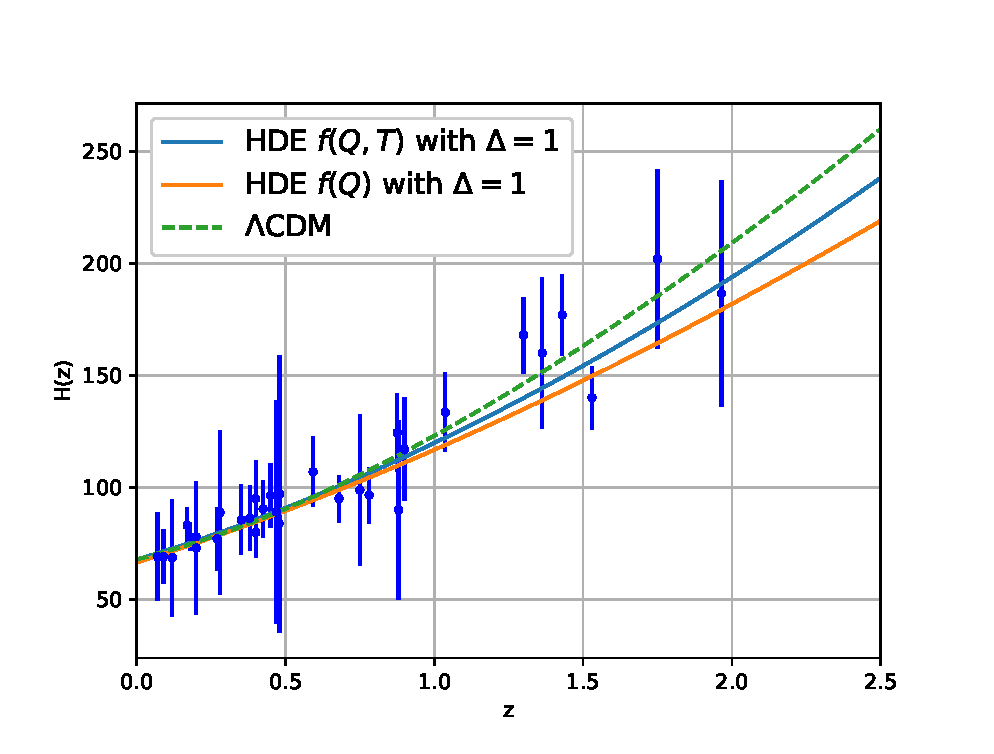
\includegraphics[width=0.45\textwidth]{./pic/H-z_relation.eps}}
    \subfigure[name2]{
    \label{Fig.sub.2}
    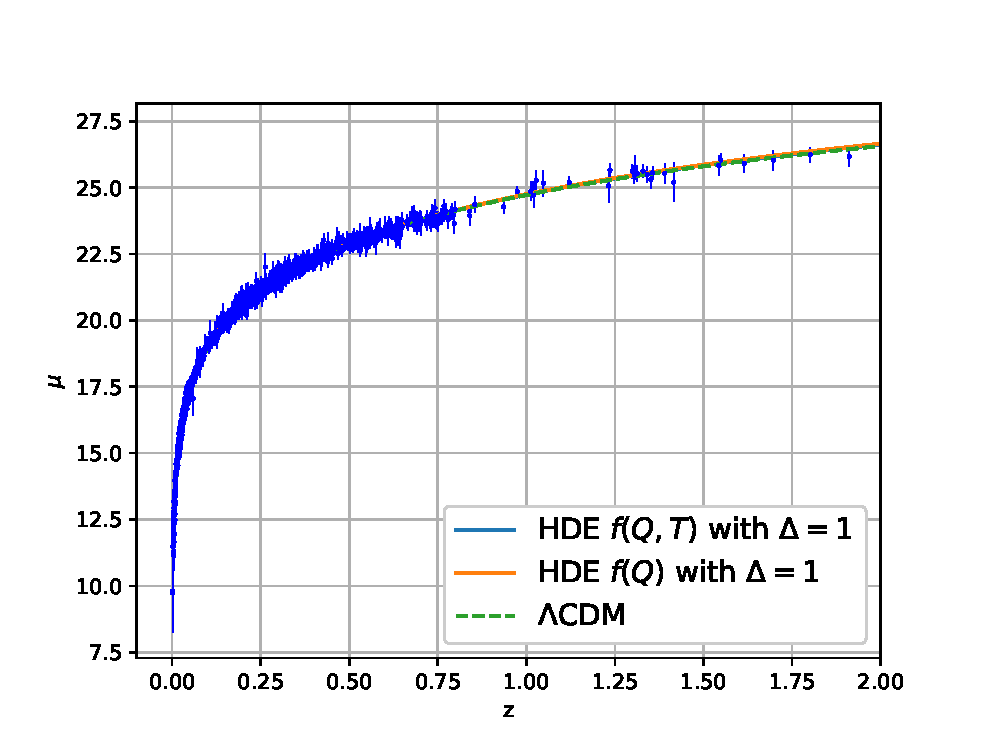
\includegraphics[width=0.45\textwidth]{./pic/mu-z_relation.eps}}
    \caption{Main name}
    \label{Fig.main}
\end{figure}

\begin{figure}[h]
    \centering
    \subfigure[name1]{
    \label{Fig2.sub.1}
    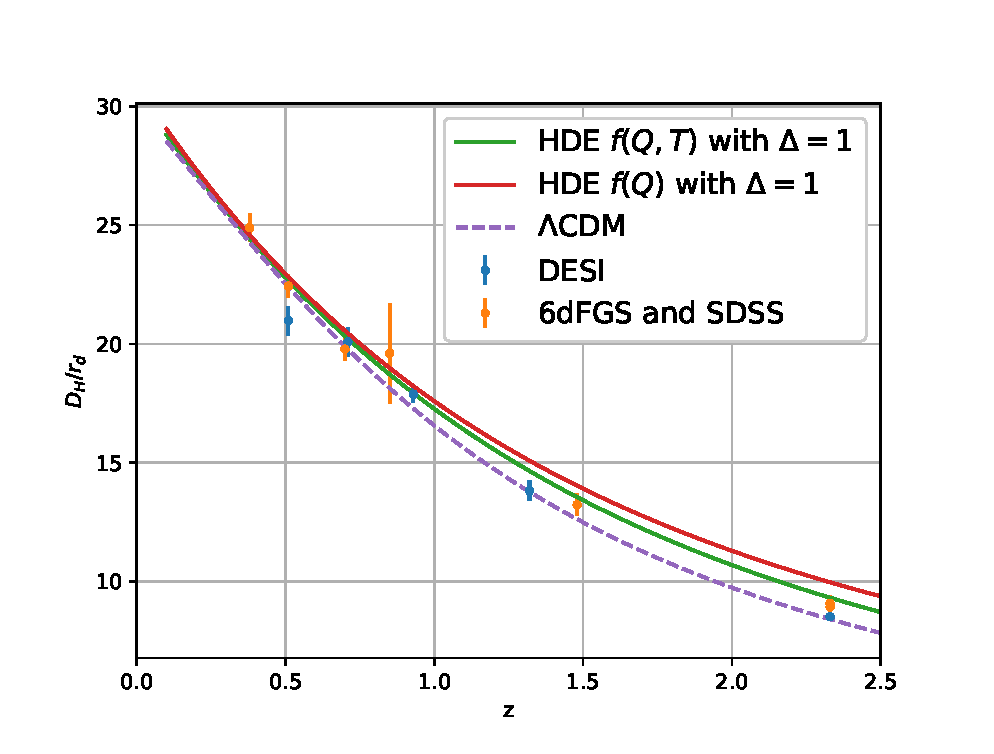
\includegraphics[width=0.3\textwidth]{./pic/DH-z_relation.eps}}
    \subfigure[name2]{
    \label{Fig2.sub.2}
    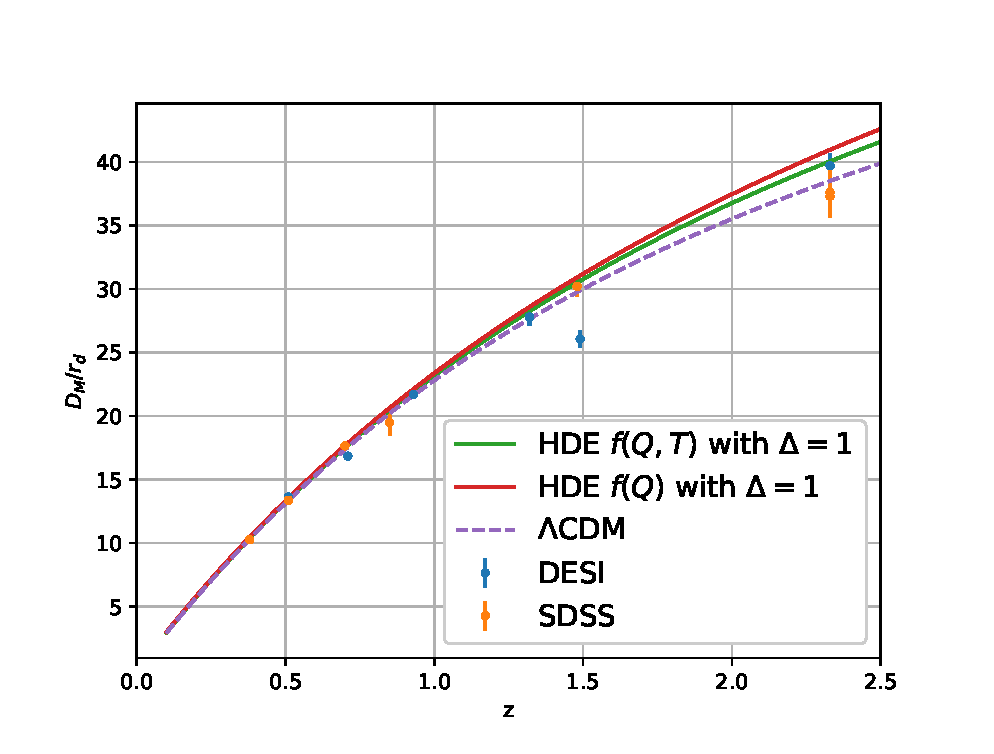
\includegraphics[width=0.3\textwidth]{./pic/DM-z_relation.eps}}
    \subfigure[name3]{
    \label{Fig2.sub.3}
    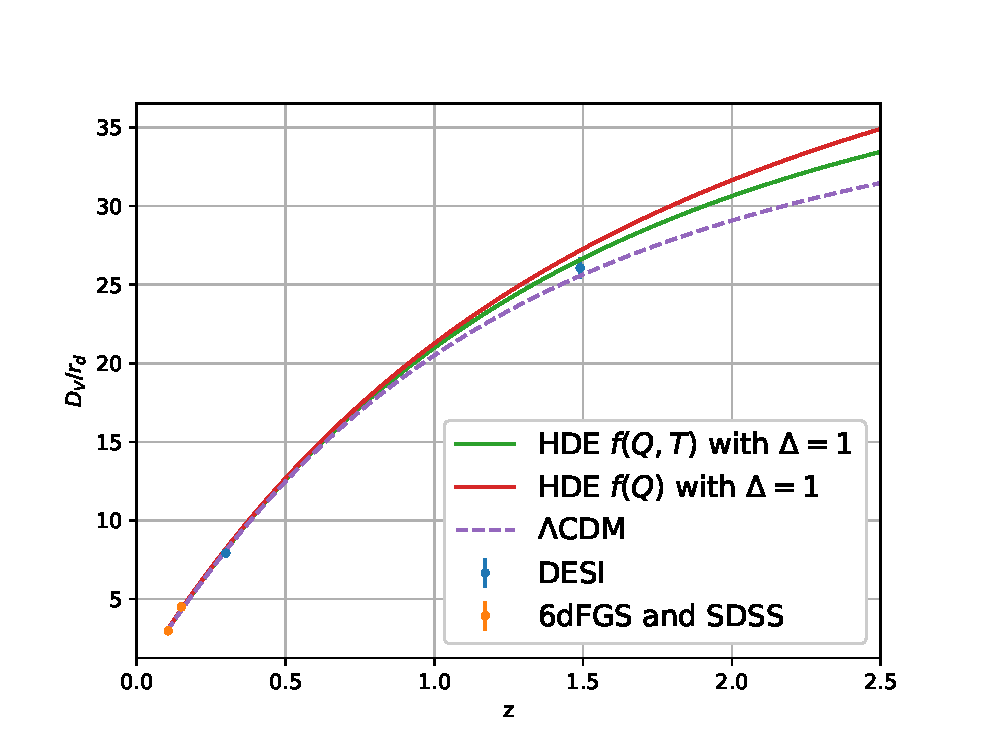
\includegraphics[width=0.3\textwidth]{./pic/DV-z_relation.eps}}
    \caption{Main name}
    \label{Fig2.main}
\end{figure}


\begin{figure}
    \centering
    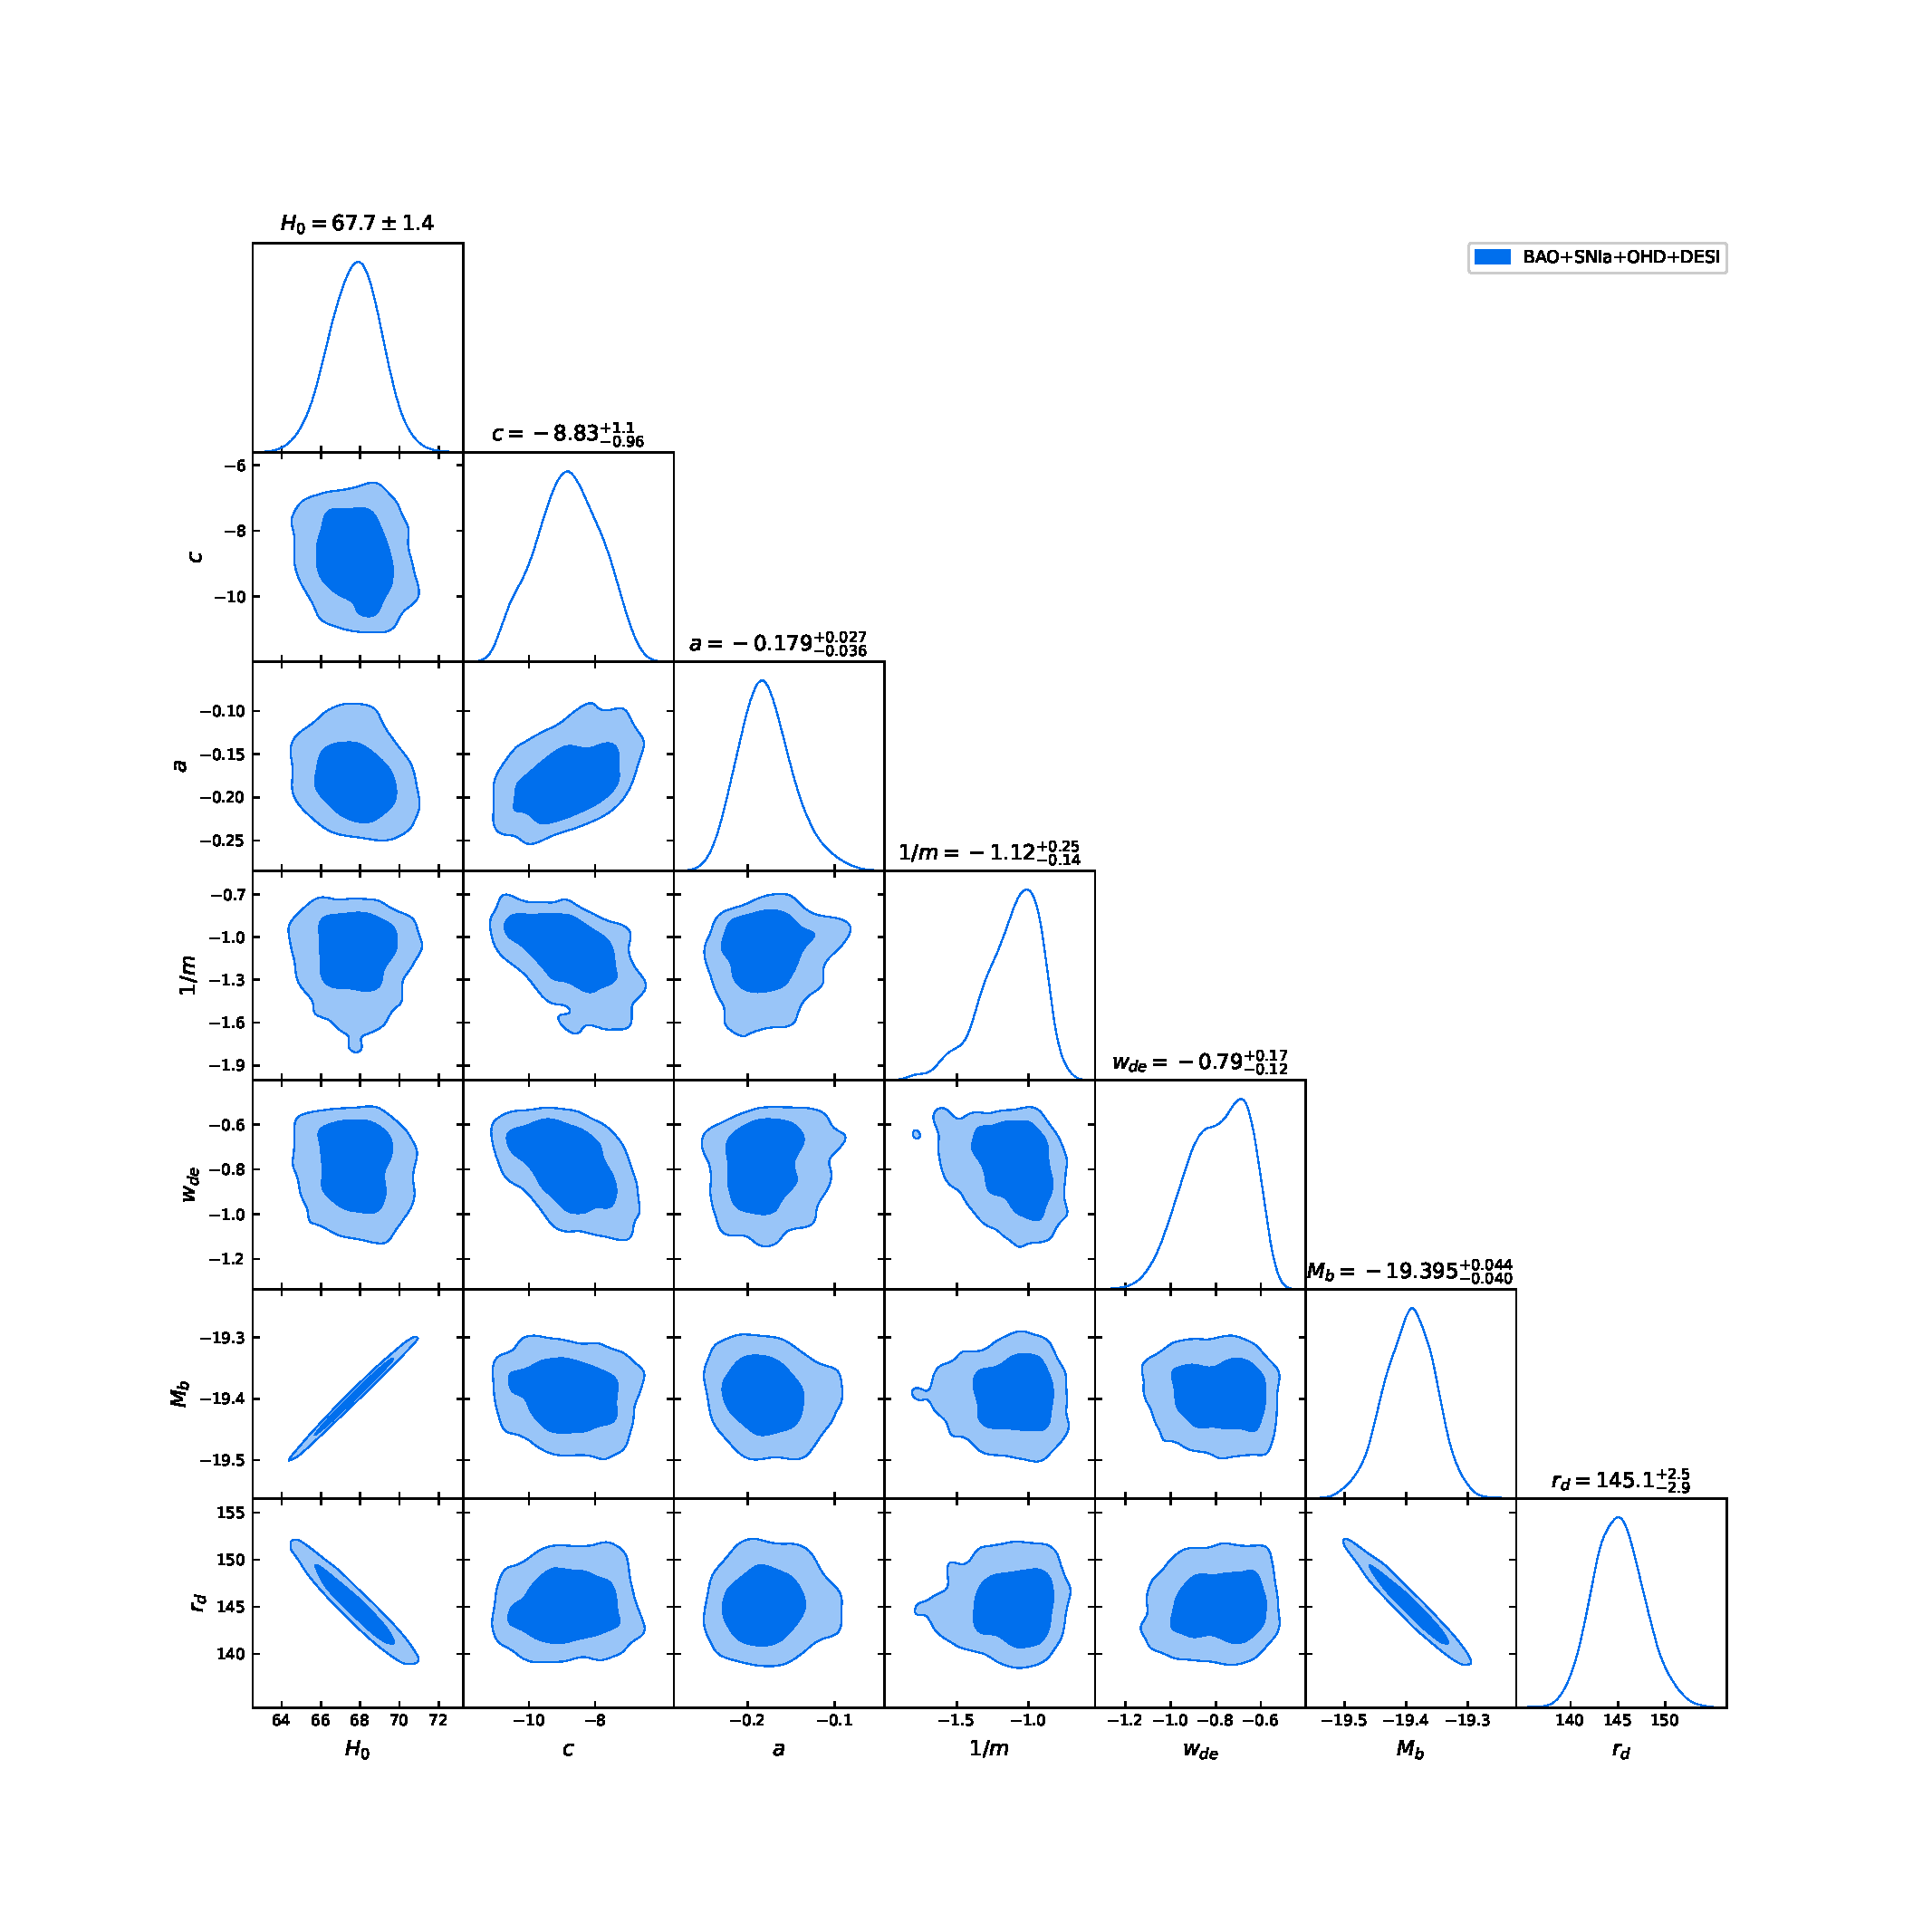
\includegraphics[width=1\linewidth]{./pic/getdist.eps}
    \caption{\label{fig:constraint} The 1$\sigma$ and 2$\sigma$ confidence contours and the 1D posterior distributions obtained from MCMC constraint of HDE in $f(Q,T)$ gravity using BAO+SNIa+OHD+DESI data}
\end{figure}
The results show that our results may alleviate the Hubble tension



\section{Conclusion}

In this paper, we discuss the evolution of holographic dark energy in the context of a non-metric modified gravity theory $f(Q,T)$. While this may seem like an overcomplicated assumption, in reality, if we live in a non-metric space (such as Weyl-Cartan geometry) rather than a Riemannian space, we cannot simply assume that dark energy no longer exists as a fluid. Instead, we continue to treat it as one of the driving forces behind cosmic acceleration, even in such a complex universe. 

We consider holographic dark energy due to its solid theoretical foundation and its interpretation as an extension of the holographic principle in cosmology. It provides a compelling explanation for the origin of dark energy, which arises from the entanglement entropy of the cosmic horizon. To refine our model, we explore a generalized version of holographic dark energy, known as Barrow holographic dark energy, which may better capture quantum corrections. For the infrared cutoff, we choose the Hubble horizon, as it is the simplest and most natural choice, although other horizons could also be considered.

For analytical simplicity, we focus on a few toy models that allow us to explore certain special cases: $\Delta=0$ for the loosest constraints and $\Delta=1$ for the tightest limits on energy density, while discussing the potential effects of non-minimal matter coupling.

To validate the model, we performed parameter estimation using recent supernova data, BAO data, and direct measurements of the Hubble parameter. By employing the MCMC method, we obtained estimates for the model parameters. Our results show that the model can effectively alleviate the Hubble constant tension. Specifically, we find that the Hubble constant is ..., in agreement with the standard cosmological model's result of .... We also study the evolution of the universe under this model and observe that the deceleration factor and the effective equation of state parameter indicate accelerated expansion, consistent with current observations.

Although this model is not yet conclusive—due to the introduction of numerous parameters and significant assumptions—it provides an interesting framework for thinking about cosmic evolution. The results and analysis presented here offer valuable insights, and further exploration of more complex scenarios will be necessary in future studies.

\appendix

\section{Appendix information}



\bibliography{sample631}{}
\bibliographystyle{aasjournal}


\end{document}

